Models are often used to explore what-if scenarios, such as scenarios of ecosystem management strategies or climate change. In general, a scenario is defined by a certain setting of model inputs. At minimum you define one standard and one alternative scenario.

In this chapter you will find out how to set up scenarios for your model. As scenarios are meant to be compared, it will also be demonstrated how you can carry out numerical analysis on the simulation output in R .

\section{Setting model scenarios}

We will define four scenarios for the butterfly model that we worked on earlier (\filenameexplained{book/butterfly2.box}). As you can see only little has changed in the box script to enable it to run scenarios:

\lstset{numbers=left}
\begin{boxscript}
// scenarios1.box
Simulation sim {
  .steps = 180
  Scenarios scenarios {
    .fileName = "scenarios/weather.txt"
  }
  Calendar calendar {
    .initialDateTime = 1/5/2009
  }
  Records weather {
    .fileName = scenarios[FileName]
  }
  Box butterfly {
    Stage egg {
      .initial = 100 
      .duration = 140
      .timeStep = ./time[step]
      DayDegrees time {
        .T0 = 5
        .T = weather[Tavg]
      }
    }
    Stage larva {
      .inflow = ../egg[outflow]
      .duration = 200
      .timeStep = ./time[step]
      DayDegrees time {
        .T0 = 8
        .T = weather[Tavg]
      }
    }
    Stage pupa {
      .inflow = ../larva[outflow]
      .duration = 100
      .timeStep = ./time[step]
      DayDegrees time {
        .T0 = 10
        .T = weather[Tavg]
      }
    }
    Stage adult {
      .inflow = ../pupa[outflow]
      .duration = 28
      .timeStep = 1
    }
  }
  OutputR {
    PageR {
      .xAxis = calendar[date]
      PlotR {
        .ports = *[content]
        .ggplot = "geom_line() + 
                   scale_x_datetime(
                     breaks = date_breaks('months'),
                     labels = date_format('%\%%b')
                   )"      
      }
    }
  }
}
\end{boxscript}
\lstset{numbers=none}

Scenarios are defined through a \code{Scenarios} box (lines 4-6). Since it defines inputs for boxes further down in the script, you should always put it as the first box inside the \code{Simulation} box. A \code{Scenarios} box takes one input, namely \code{fileName} (line 5). In this case it refers to a text file (\filename{\inputfolder/book/scenarios/weather.txt}) with the following content:

\lstset{numbers=left}
\begin{textfile}
FileName
"scenarios/flakkebjerg 2009 Tavg.txt"
"scenarios/braunschweig 2009 Tavg.txt"
"scenarios/geneva 2009 Tavg.txt"
"scenarios/ljubljana 2009 Tavg.txt"
\end{textfile}
\lstset{numbers=none}

\begin{figure}
\centering
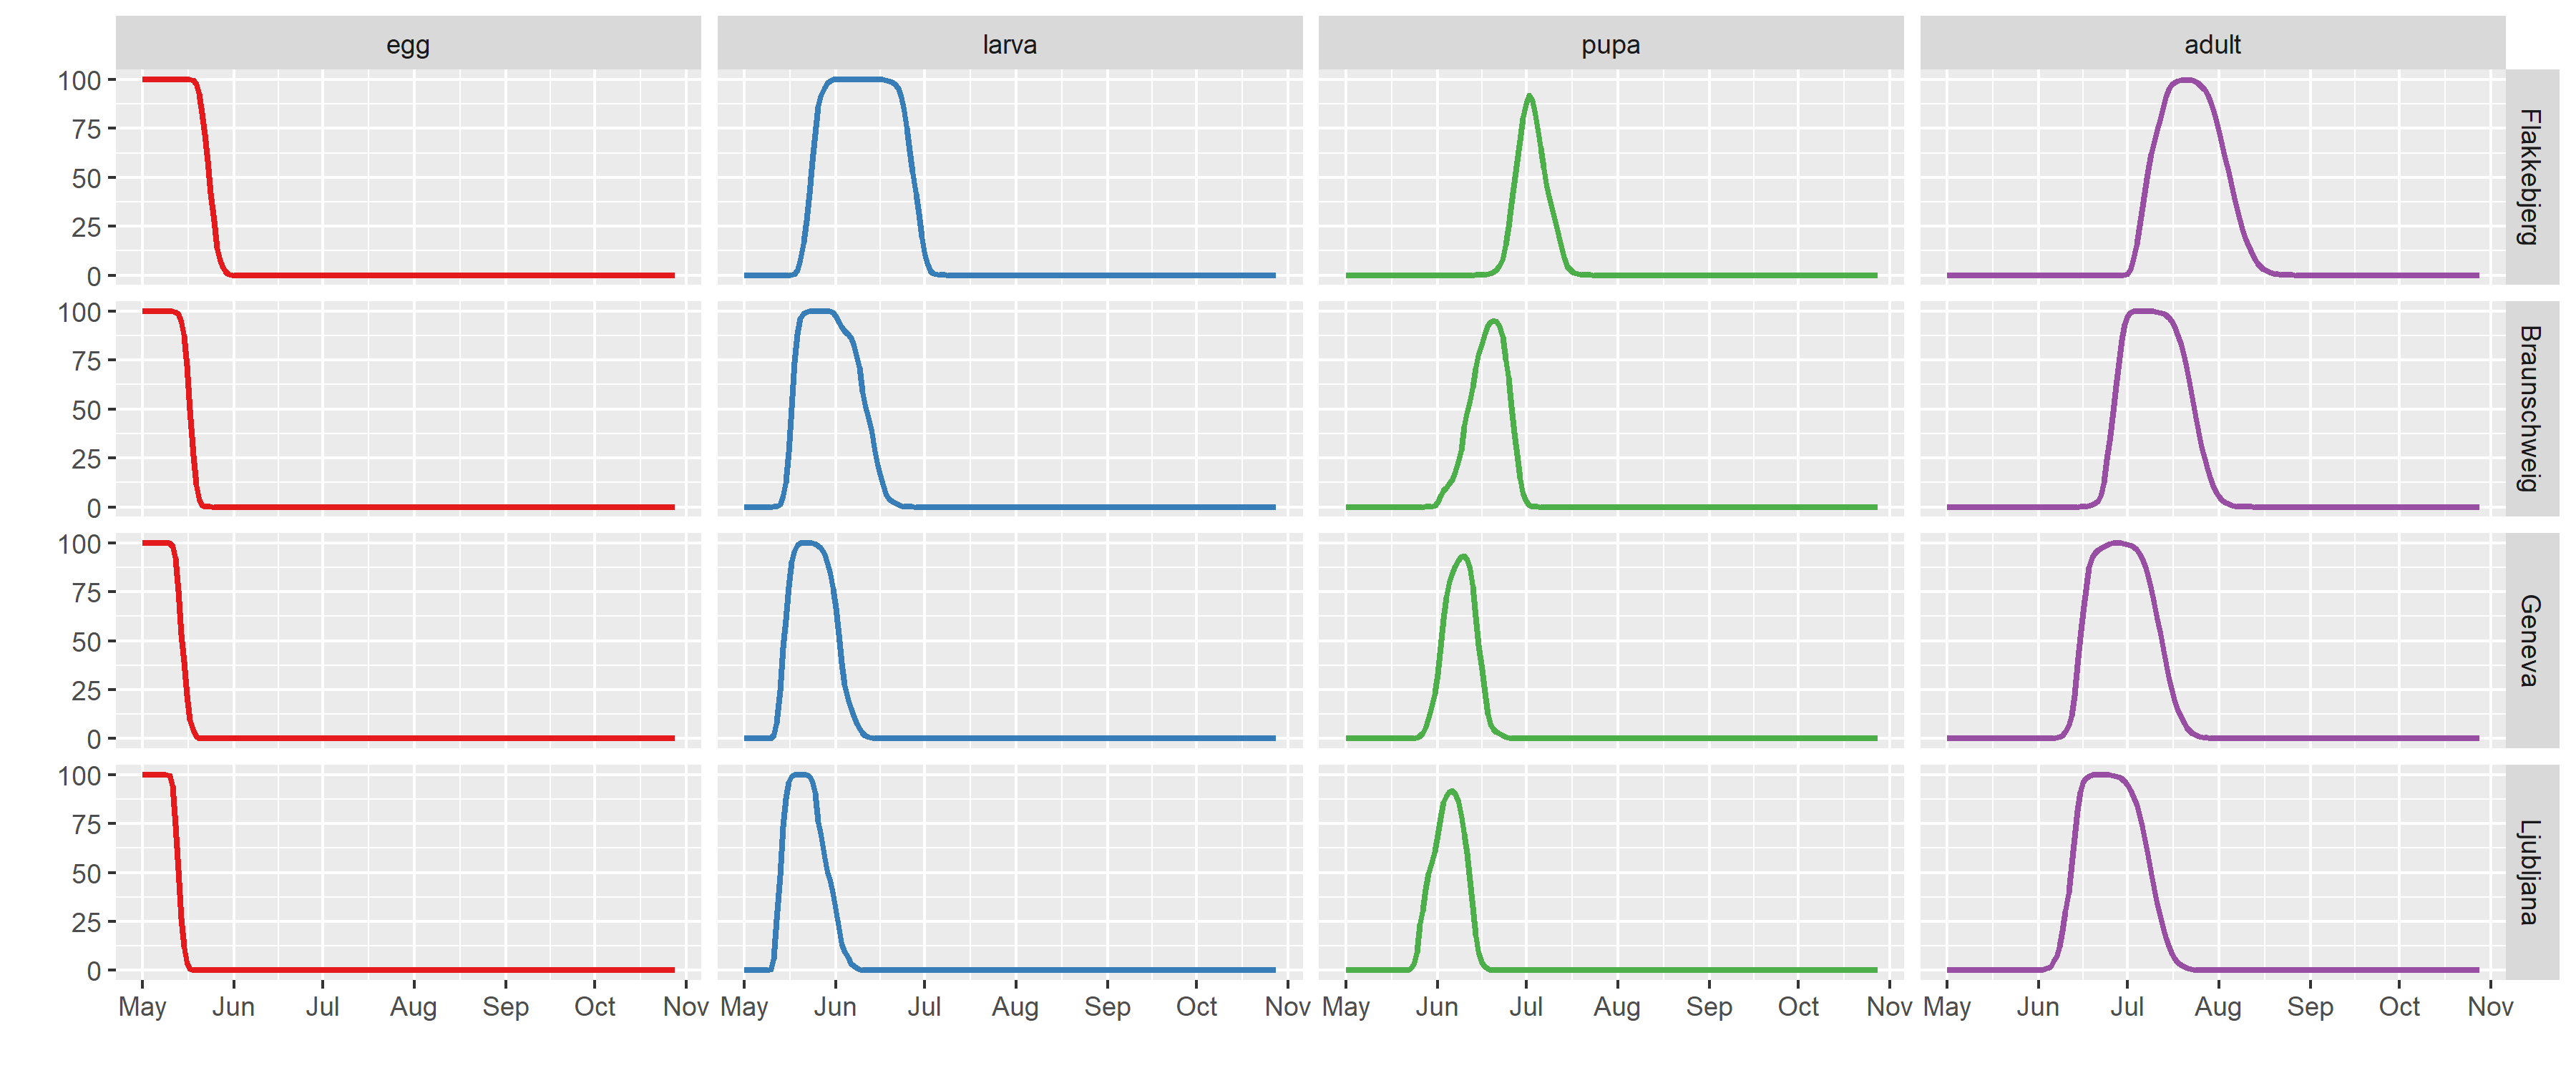
\includegraphics[width=\textwidth]{graphics/scenarios2}
\caption{Butterfly phenology at four different locations in Europe, numbered 1-4. Generated by the \filename{\inputfolder/book/scenarios2.box} script.}
\label{fig:scenarios1-2}
\end{figure}

The text file must be column-oriented with columns separated by whitespace (\eg\ tab stops) and with the first line containing names for each column. This is the same format used by the \code{Records} box (which we have used already to handle weather input) and also commonly for text file input into R. In this example, it contains just one column named \code{FileName}. It has four rows naming different weather files. You should verify that these four files in fact exist in your \filename{\inputfolder/book/scenarios} folder. The file names are in apostrophes because they are strings (\ie\ text) which might contain spaces (as they do in this case). Without the apostrophes, the file names would be broken into different columns at the spaces. Other data types, such as numbers, you can always write without apostrophes.

The \code{Scenarios} box is a tyranic one as it directs the \code{Simulation} box to run iteratively, one run for each row in the scenarios input file (four rows, in this case). You cannot tell this from the box script because the functionaliy is implemented in the \CPP\ code (where you can fint it in the \code{initialise} method in the \filename{scenarios.cpp} file). For each iteration, the \code{Scenarios} box will advance one line in its input file. Other boxes in the script can grab the current values from the scenarios input file, thus effectuating the scenario set-up. In the \filename{scenarios1.box} script, this happens in line 11 only, where the \code{fileName} input is set for \code{weather}. A \code{Scenarios} box creates an output port for each column in the scenarios file, giving the output the name of the column heading, here \code{FileName}.

For a \code{Records} box to work with scenarios, the weather files must all have the same format in terms of the number of columns and column names. The four weather files used here were polished for this purpose, as you can verify by inspecting them with a text editor.

The output is automatically ordered to yield one row of panels for each iteration (\iref{fig:scenarios1-2}). The scenarios were ordered on a north-south gradient which is reflected in the phenology shifting to the left, as you scan down the panels.

\section{Adjusting plots}
If you run \filename{scenarios1.box} and compare the output on your screen with that shown in \iref{fig:scenarios1-2}, you will notice a slight difference. By default, iterations are simply identified by the iteration number shown on the righthand panel captions. In 
\iref{fig:scenarios1-2} these numbers have been replaced by the names of the scenario locations. This is achieved by the \filename{scenarios2.box} script.

In general, to take finer control of the output generated by the box script, we need to write an R script. The R script is linked to the box script through the \code{OutputR} box. In \US\ you can retrieve information on \code{OutputR} using the \code{help} command. Here you find, among others, the \code{begin} and \code{end} inputs:

\begin{rdialog}
> help OutputR
:
Input:
.begin | scripts/begin.R | ...
.end   | scripts/end.R   | ...
:
>
\end{rdialog}

The \code{begin} and \code{end} ports set the R scripts, that will run before and after, respectively, the R script generated by \US\ from your box script. The default scripts (\code{begin.R} and \code{end.R}) can be found in the \filename{\inputfolder/scripts} folder. To change the design of the output plot, we need to replace the standard \filename{end.R} script with our own. As a starting point, let's study the code of the default \filename{end.R} script. It contains just two lines of R code:

\lstset{numbers=left}
\begin{rscript}
sim = read_output(output_file_name)
plot_all(sim)
\end{rscript}
\lstset{numbers=none}

First the \code{sim} data frame is read from the output file generated by \US\ (line 1). Then \code{sim} is used as an input to the \code{plot_all} function (line 2). All we need to do is to put some code between these two lines, that replaces the iteration numbers with location names. Remember: Do not change the default \filename{end.R} script. Instead, create a new R script in the same folder as your box script.

If you investigate the \code{sim} data frame in R (first run the \filename{scenarios1.box} script then copy the clipboard into R as usual), you will find that the iteration number is kept in the \code{iteration} column of \code{sim}:

\begin{rdialog}
> head(sim[,1:4])
  iteration       date egg.content larva.content
1         1 2009-05-01         100             0
2         1 2009-05-02         100             0
3         1 2009-05-03         100             0
4         1 2009-05-04         100             0
5         1 2009-05-05         100             0
6         1 2009-05-06         100             0
> class(sim$iteration)
[1] "integer"
> unique(sim$iteration)
[1] 1 2 3 4
> 
\end{rdialog}

So, \code{iteration} is of the integer class and takes on the values 1 to 4. This is as expected. We will now change this, converting \code{iteration} to a factor and replacing the four levels with the location names (\filename{\inputfolder/book/scenarios/end-locations.R}):
\lstset{numbers=left}
\begin{rscript}
# Replace iteration numbers with location names
sim = read_output(output_file_name)
sim$iteration = factor(sim$iteration)
levels(sim$iteration) = 
  c("Flakkebjerg", "Braunschweig", 
    "Geneva", "Ljubljana")
plot_all(sim)
\end{rscript}
\lstset{numbers=none}

Here, line 1 and 7 were retained from the original \filename{end.R} script. Lines 2-6 do the conversion from numbers to text. To effectuate this R script we set the \code{end} port of the \code{OutputR} box, like this:

\begin{boxscript}
// From scenarios2.box
OutputR {
  .end = "scenarios/end-locations.R"
  PageR {
  :
  }
}
\end{boxscript}

The improved output is the one shown in \iref{fig:scenarios1-2}.

\section{Analysing model output}
We will now proceed to analyse the simulation output further, aiming to
produce a plot that reveals the expected period when butterflies will be flying
at the four locations. For this purpose we change the \code{end} R script further (\filename{\inputfolder/book/scenarios/end-analysis.R}):

\lstset{numbers=left}
\begin{rscript}
sim = read_output(output_file_name)
sim$Location = factor(sim$iteration)
levels(sim$Location) = c("Flakkebjerg", "Braunschweig", 
                         "Geneva", "Ljubljana")

sim$DayNum = yday(sim$date)

to_date = function(x) {
  dmy("31/12/2008") + days(round(x))
}

stats = function(df) {
  f = approxfun(df$outflowTotal, df$DayNum)
  data.frame(From = to_date(f(10)), 
             Median = to_date(f(50)), 
             To = to_date(f(90)),
             Duration = to_date(f(90)) - to_date(f(10)))
}

A = ddply(sim, .(Location), stats)
print(A)

P = ggplot(A) +
  geom_point(aes(y=Location, x=Median, colour=Location), 
             size=3) +
  geom_errorbarh(aes(y=Location, x=Median, 
                     xmin=From, xmax=To, 
                     height=0, colour=Location), 
                     size=1.3) +
  xlab("Butterflies flying") + ylab("") +
  theme(legend.position="none")

print(P)
\end{rscript}
\lstset{numbers=none}

Here, we create a new column \code{Location} to hold the location name (lines 2-4). In another column \code{DayNum} we put the day number computed from \code{date} (line 6). \textit{Vice versa}, the \code{to_date} function converts a day number to the corresponding date in the year 2009 (lines 8-10).

The \code{stats} function does the hard work computing statistics on the data frame (\code{df}) it takes as input (lines 12-18). The \code{ddply} function is used to call \code{stats} repeatedly, once for each level of \code{Location}, \ie\ four times in our case (line 20). As a result \code{df} in \code{stats} will hold a subset of \code{sim}, when \code{stats} is called from \code{ddply}. Thus \code{stats} will handle one location at a time.

The \code{approxfun} function is an R function with a surprising kind of output. It outputs a function! Here we give that function the name \code{f} (line 13). To use \code{approxfun} you give it a vector of $x$-values and a vector of $y$-values.  Here we use the accumulated emergence of adult butterflies (\code{df\$outflowTotal}) for $x$ and the day of the year for $y$. Based on this information, the generated function \code{f} will calculate $y$ from a given $x$ by linear interpolation. In effect, we can ask \code{f} on what day of the year a certain total emergence was achieved. This day of the year (1-365) we can then convert to a proper date using our \code{to_date} function.

The \code{stats} function returns a data frame with just one row (lines 14-17) and the following columns: \code{From}, \code{Median} and \code{To} representing the 10\%, 50\% and 90\% percentiles of emergence, respectively; and \code{Duration} which holds the number of days between \code{From} and \code{To}. Note that we get, \eg\ the 10\% percentile when 10 butterflies have emerged, because we have a total of 100 individuals.

To make use of the \filename{end-analysis.R} script we put it as the \code{end} input to the \code{OutputR} box (line 3):

\lstset{numbers=left}
\begin{boxscript}
// From scenarios3.box
OutputR {
  .end = "scenarios/end-analysis.R"
  OutputText { 
    .ports = (calendar[date] adult[outflowTotal])
  }
}
\end{boxscript}
\lstset{numbers=none}

Since we now produce all the plot ourselves, we no longer need the automatic plots produced by \code{PageR} and \code{PlotR}. Instead we use the \code{OutputText} box which does nothing but write the selected \code{ports} (line 5) to the output text file. This is the very text file that we subsequently read into the \code{sim} data frame in the first line of the \filename{end-analysis.R} script:
\begin{rscript}
sim = read_output(output_file_name)
\end{rscript}
\US\ has taken care that the variable \code{output_file_name} holds the right file name and path.

Finally, we are rewarded for our efforts by the plot shown in \iref{fig:scenarios3}. Our end script also prints the contents of the \code{A} data frame at the R prompt:

\begin{rscript}
    Location       From     Median         To Duration
 Flakkebjerg 2009-07-30 2009-08-06 2009-08-14  15 days
Braunschweig 2009-07-19 2009-07-25 2009-07-31  12 days
      Geneva 2009-07-08 2009-07-14 2009-07-21  13 days
   Ljubljana 2009-07-04 2009-07-10 2009-07-17  13 days
\end{rscript}

Clearly, location along the north-south gradiant has larger impact on the time of flying than on the duration of the flying period.

\begin{figure} [t]
\centering
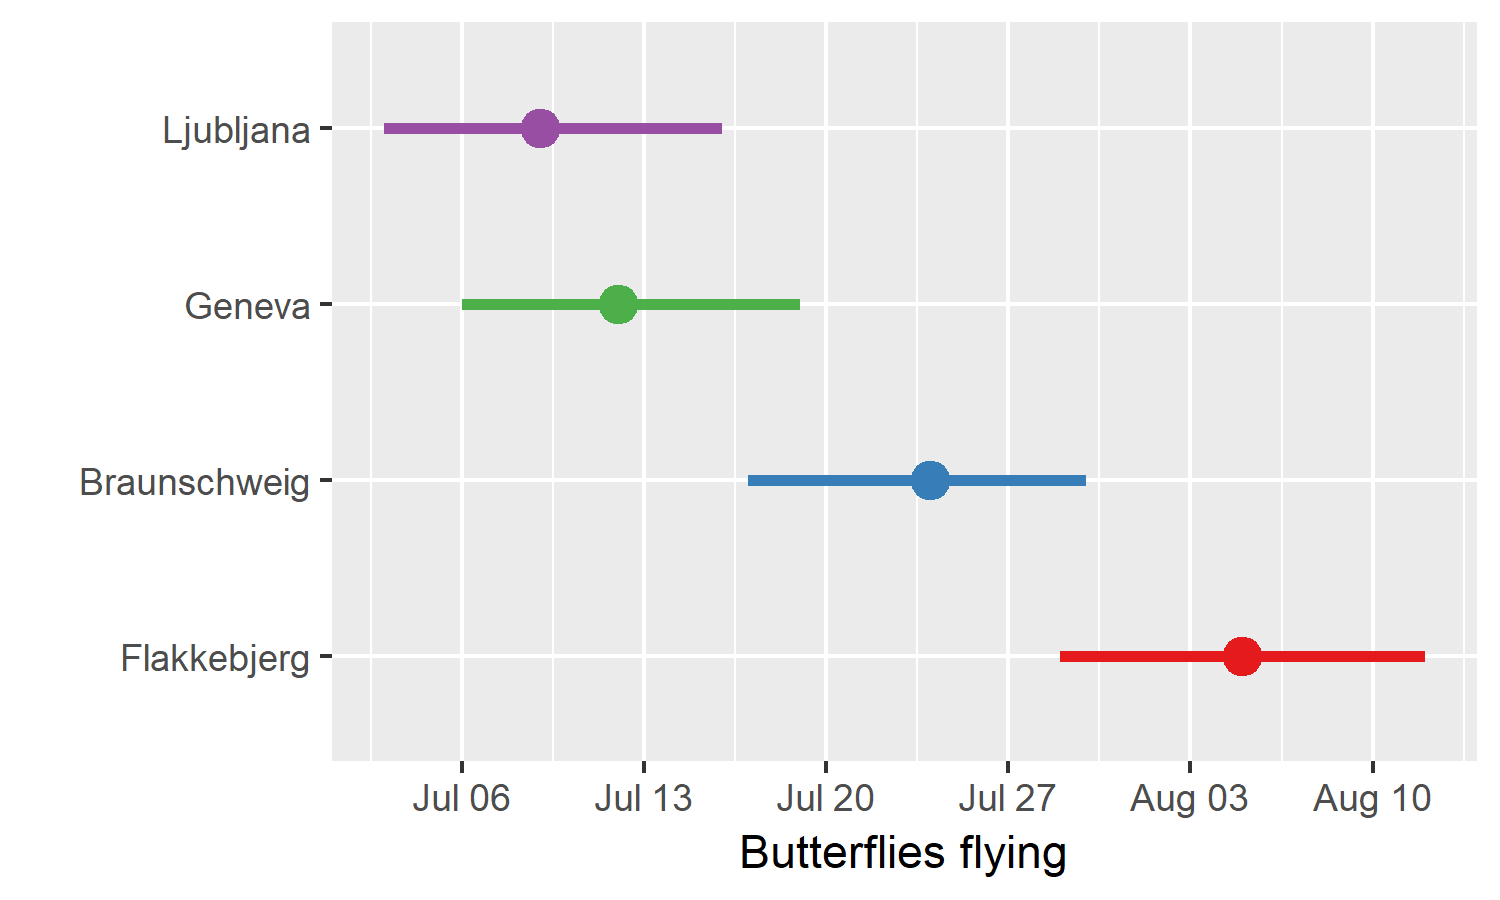
\includegraphics[width=\textwidth]{graphics/scenarios3}
\caption{Butterfly flying phenology at four different locations in Europe. Generated by the \filename{\inputfolder/book/scenarios3.box} script.}
\label{fig:scenarios3}
\end{figure}

 